\begin{center}
	\huge \textbf{Il modello PRNR}
	
	\rule{7cm}{0.4pt} 
	
	\LARGE Un modello matematico per la Rivoluzione Francese
	
	\vspace{20pt}
	
	\LARGE \textbf{Cristina Caprioglio, Luca Morelli}
	
	\vspace{5pt}
	
	\LARGE 20 Dicembre 2022
	
	\vspace{20pt}
 
	\normalsize\textbf{Abstract:}\\
\end{center}
Scrivere un Abstract.

\vspace{20pt}

\section*{Introduzione}
Per questo progetto abbiamo cercato di modellizzare lo scoppio di una rivoluzione. Per farlo ci siamo serviti del modello multicompartimentale, che ci ha permesso di descrivere le possibili transizioni di stato delle persone del nostro sistema. In particolare, abbiamo diviso la popolazione iniziale tra poveri e ricchi: i primi potevano transire nello stato "Rivoluzionari" e i secondi in quello "Reazionari". Sia i rivoluzionari che i reazionari potevano tornare a far parte rispettivamente dei poveri e dei ricchi. Le transizioni sono descritte da diversi parametri spiegati nel dettaglio nel seguente paragrafo, ma entrambe dipendono dal numero di individui presenti nei vari compartimenti. Chiaramente il numero di persone per ogni settore varia con il tempo: nella parte di simulazione questa variazione è stata considerata discreta, mentre nella fase di integrazione continua. 
É bene tener presente che ogni individuo appartenente ad un settore, a parità di condizioni con altri suoi simili, ha la stessa probabilità di cambiare stato.
\section{Il sistema e il modello}
Come precedentemente detto, vogliamo studiare la dinamica di una popolazione composta da vari membri, in numero elevato, che differiscono l'uno dall'altro per il loro reddito. Queste differenze, sotto determinate condizioni, possono spingere gli individui appartenenti alla categoria più povera ad insorgere. Questa insurrezione può a sua volta portare alcuni tra i più abbienti a reprimerla con l'uso della forza.\\

Per modellizzare una popolazione eterogenea abbiamo deciso di suddividerla in due categorie, \textbf{Poveri} e \textbf{Nobili}, per le quali si considera un reddito medio caratteristico di ciascuna categoria.\\
Ogni membro di questa popolazione può decidere, in base a vari fattori, di far uso della violenza per far valere le esigenze della propria categoria. Abbiamo considerato che ogni individuo può trovarsi o in uno stato di normalità o in uno stato eccitato: un membro della categoria dei Poveri nello stato \textbf{Normale} $(N_P)$ può transire allo stato di \textbf{Rivoluzionario} $(R)$, mentre un membro della categoria dei Nobili nello stato \textbf{Normale} $(N_N)$ può transire allo stato di \textbf{Reazionario} $(\bar{R})$. All'interno della stessa categoria può avvenire anche la transizione inversa, come mostrato in figura (\ref{fig:CompartmentScheme}).\\
\begin{figure}[H]
	\centering
	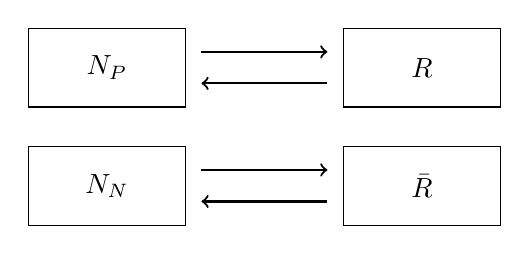
\begin{tikzpicture}
        \draw[draw=black] (0,0) rectangle (2,1);
		\draw[->, thick] (2.2,.7) -- (3.8,.7);
		\draw[<-, thick] (2.2,.3) -- (3.8,.3);
		\draw[draw=black] (4,0) rectangle (6,1) ;
		\node at (5,0.5) {$\bar{R}$};
		\node at (1,0.5) {$N_N$};
		\draw[draw=black] (0,1.5) rectangle (2,2.5);
		\draw[->, thick] (2.2,2.2) -- (3.8,2.2);
		\draw[<-, thick] (2.2,1.8) -- (3.8,1.8);
		\draw[draw=black] (4,1.5) rectangle (6,2.5) ;
		\node at (5,2) {$R$};
		\node at (1,2) {$N_P$};
    \end{tikzpicture}
	\label{fig:CompartmentScheme}
	\caption{Schema a compartimenti delle categorie delle persone. Con le frecce sono evidenziate le transizioni di stato che un individuo può effettuare.}
\end{figure}
Per questa modellizazione abbiamo deciso, come è consueto fare, di non  considerare le possibili fluttuazioni del numero totale di individui dovuti alla morte e alla nascita di persone, inoltre abbiamo considerato che un individuo non possa transire dalla categoria di Povero a quella di Nobile. Questa scelta è giustificata dall'osservazione che, seppur possibili, tali transizioni in genere sono estremamente rare. Queste considerazioni ci hanno quindi permesso di identificare 3 vincoli da imporre al modello:
\begin{equation}
    \frac{N_P(t)+R(t)}{N_P(0)+R(0)+N_N(0)+\bar{R}(0)}=F_P \quad\:\frac{N_N(t)+\bar{R}(t)}{N_P(0)+R(0)+N_N(0)+\bar{R}(0)}=F_N \quad\: F_P+F_N=1 
	\label{vincoli}
\end{equation}
dove $F_P$ e $F_N$ sono rispettivamente le frazioni di individui Poveri e Nobili sulla popolazione totale.\\

Dobbiamo ora identificare quali equazioni regolino la dinamica del sistema. Per fare ciò abbiamo ragionevolmente supposto che:
\begin{itemize}
	\item un Povero possa transire allo stato di Rivoluzionario o di sua spontanea iniziativa (nata della sua condizione disagiata) oppure incontrando un rivoluzionario che lo convinca ad insorgere
	\item un Rivoluzionario, incontrando dei Reazionari, possa essere convinto a non perseguire più la sua causa ritornando allo stato Normale
	\item un Nobile, incontrando un rivoluzionario, possa in risposta decidere di diventare un Reazionario
	\item un Reazionario, vedendo diminuire il numero di Rivoluzionari (e quindi aumentare quello di Poveri allo stato normale), possa decidere di ritornare anch'esso allo stato normale  
\end{itemize}
Se consideriamo un tempo $\Delta t$ possiamo esprimere le variazioni del numero di ogni compartimento, tenendo conto delle precedenti considerazioni, con:

\begin{flalign*}
      &R(t+\Delta t)-R(t)=\Gamma N_P(t) \frac{R(t)}{N_{tot}}\Delta t+\gamma N_P(t)\Delta t-\bar{\Gamma}R(t)\frac{\bar{R}(t)}{N_{tot}}\Delta t\\\nonumber
	  &\bar{R}(t+\Delta t)-\bar{R}(t)=\alpha N_N(t)\frac{R(t)}{N_{tot}}\Delta t-\beta \bar{R}(t)\frac{N_P(t)}{N_{tot}}\Delta t\\\nonumber
	  &N_P(t+\Delta t)-N_P(t)=-(R(t+\Delta t)-R(t))\\\nonumber
	  &N_N(t+\Delta t)-N_N(t)=-(\bar{R}(t+\Delta t)-\bar{R}(t))\\\nonumber
\end{flalign*}	
$ \Gamma $ é un parametro che indica la probabilità che un povero diventi rivoluzionario in seguito al contatto con i membri di quest'ultima categoria, mentre invece $ \bar{\Gamma} $ indica la probabilità che un rivoluzionario, per via della presenza di reazionari, decida di abbandonare la propria causa e torni quindi allo stato "Normale". $\gamma$, diversamente dai primi due, riguarda la probabilità che un povero passi da "Normale" a rivoluzionario per volontà propria, senza influenze esterne. $ \alpha $ e $ \beta $ sono i due parametri relativi alla variazione dei reazionari: il primo riguarda la probabilità che un nobile diventi reazionario per via dell'aumento dei rivoltosi, mentre il secondo che un reazionario torni "Normale" in seguito alla crescita del numero dei poveri in stato "Normale" (e conseguente diminuzione di rivoluzionari). \\
Prima di procedere nello studio del modello, al fine di semplificarlo, riscaliamo le variabili dividendole per $ N_{tot}$, che indica la popolazione totale, ovvero la somma di tutti i poveri e di tutti i ricchi. In questo modo otteniamo il seguente set di espressioni:  

\begin{flalign*}
	&R'(t+\Delta t)-R'(t)=\Gamma N'_P(t)'R'(t)\Delta t+\gamma N'_P(t)\Delta t-\bar{\Gamma}R'(t)\bar{R'}(t)\Delta t\\\nonumber
	&\bar{R'}(t+\Delta t)-\bar{R'}(t)=\alpha N'_N(t)R'(t)\Delta t-\beta \bar{R'}(t)N'_P(t)\Delta t\\\nonumber
	&N'_P(t+\Delta t)-N'_P(t)=-(R'(t+\Delta t)-R'(t))\\\nonumber
	&N'_N(t+\Delta t)-N'_N(t)=-(\bar{R'}(t+\Delta t)-\bar{R'}(t))\\\nonumber
\end{flalign*}	
con 
\begin{equation*}
	N'_{P}(t)=\frac{N_{P}(t)}{N_{tot}} \qquad 	N'_{N}(t)=\frac{N_{N}(t)}{N_{tot}} \qquad	R'(t)=\frac{R(t)}{N_{tot}} \qquad	\bar{R'}(t)=\frac{\bar{R}(t)}{N_{tot}} 
\end{equation*}
Per alleggerire la notazione, dato che da questo momento in poi useremo sempre le variabili riscalate, quest'ultime perderanno il simbolo $ ' $ davanti e verranno scritte normalmente. \\
All'interno della simulazione, visto che si calcolava la probabilità di ogni singolo individuo di compiere una transizione e non la variazione nel tempo dell'intero settore, tutti i parametri (con l'eccezione di $ \gamma $) sono stati divisi per 8. Questo perchè, calcolando la probabilità che avvenga una transizione, se la prima è influenzata dalla presenza o meno di un membro appartenente ad una certa categoria, andrà moltiplicata per la probabilità di incontrarlo. Nel nostro caso, ogni persona poteva interagire solo con le 8 celle adiacenti, perciò abbiamo dovuto moltiplicare per $ \frac{1}{8} $.
\\\\ 
Per poter integrare il nostro modello abbiamo diviso ogni espressione per $ \Delta t $ e, considerando intervalli di tempo abbastanza piccoli, siamo potuti passare al continuo:
\begin{flalign*}
		&\frac{dR}{dt}=\Gamma N_P(t) R(t)+\gamma N_P(t)-\bar{\Gamma}R(t)\bar{R}(t)\\\nonumber
		&\frac{d\bar{R}}{dt}=\alpha N_N(t)R(t)-\beta \bar{R}(t)N_P(t)\\\nonumber
		&\frac{dN_{P}}{dt}= -\frac{dR}{dt}\\\nonumber
		&\frac{dN_{R}}{dt}= -\frac{d\bar{R}}{dt}\\\nonumber
\end{flalign*}
Una volta ottenute queste equazioni differenziali abbiamo potuto integrarle numericamente.\\

